\documentclass{article}

\usepackage{minted}

\usepackage[utf8]{inputenc}
\usepackage{gensymb}
\usepackage{amsfonts}
\usepackage{amsmath}
\usepackage{graphicx}
\usepackage{tabularx}
\usepackage{geometry}
\usepackage{float}
\usepackage{tikz}
\usetikzlibrary{calc}

% Adjust margins for solutions
\geometry{a4paper, margin=1in}

\title{Bearings Challenge - Worked Solutions}
\author{Solutions Guide}
\date{}

\begin{document}

\maketitle


\section{Introduction}

  \begin{enumerate}
   \item
   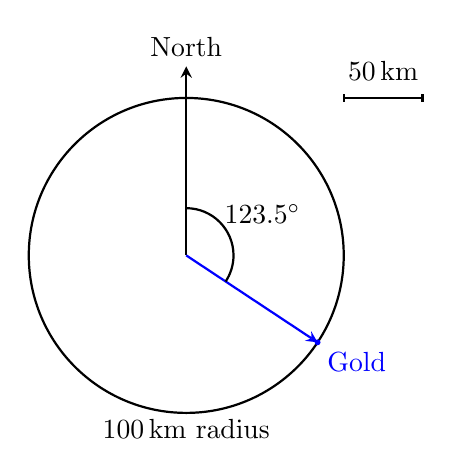
\begin{tikzpicture}[scale=1, >=stealth]

    % Parameters
    \def\R{2}            % visual radius for 100 km
    \def\bearing{123.5}
    
    % Origin
    \coordinate (O) at (0,0);
    
    % Main circle (radius = 100 km)
    \draw[thick] (O) circle (\R);
    \node at (0,-\R-0.2) {$100\,\text{km}$ radius};
    
    % North arrow
    \draw[->, thick] (O) -- (0,1.2*\R) node[above] {North};
    
    % Bearing line
    \draw[thick, blue, ->]
      (O) -- ({\R*sin(\bearing)}, {\R*cos(\bearing)});
    
    % Gold location
    \filldraw[blue]
      ({\R*sin(\bearing)}, {\R*cos(\bearing)})
      circle (0.03)
      node[below right] {Gold};
    
    % Bearing angle arc (clockwise from North)
    \draw[thick]
      (0,0.6) arc[start angle=90, end angle={90-\bearing}, radius=0.6];
    
    \node at ({1.1*sin(\bearing/2)}, {1.1*cos(\bearing/2)})
      {$123.5^\circ$};
    
    % Distance scale / key
    \begin{scope}[shift={(2.0,2.0)}]
    
    \draw[thick] (0,0) -- (1,0);
    \draw[thick] (0,-0.05) -- (0,0.05);
    \draw[thick] (1,-0.05) -- (1,0.05);
    \node[above] at (0.5,0.1) {$50\,\text{km}$};
    
    \end{scope}
\end{tikzpicture}

\item The journey describes involves travelling due South, then due east.

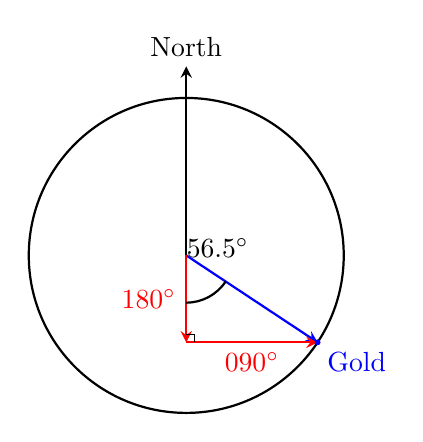
\begin{tikzpicture}[scale=1, >=stealth]

% Parameters
\def\R{2}
\def\bearing{123.5}

% Origin
\coordinate (O) at (0,0);

% Key points
\coordinate (G) at ({\R*sin(\bearing)}, {\R*cos(\bearing)});
\coordinate (S) at (0,{\R*cos(\bearing)});

% Main circle
\draw[thick] (O) circle (\R);

% North arrow
\draw[->, thick] (O) -- (0,1.2*\R) node[above] {North};

% True bearing
\draw[thick, blue, ->]
  (O) -- (G);

% First leg: South
\draw[thick, red, ->]
  (O) -- (S)
  node[midway, left] {$180^\circ$};

% Second leg: East
\draw[thick, red, ->]
  (S) -- (G)
  node[midway, below] {$090^\circ$};

% Gold
\filldraw[blue]
  (G) circle (0.03)
  node[below right] {Gold};

% Right angle marker at S
\draw (0.1,{\R*cos(\bearing)}) --
      (0.1,{\R*cos(\bearing)+0.1}) --
      (0,{\R*cos(\bearing)+0.1});

% Angle at origin: 56.5 degrees
% Angle at origin: 56.5 degrees (bottom-right)
\draw[thick]
  (O) ++(0,-0.6)
  arc[start angle=270, end angle={270+(180-\bearing)}, radius=0.6];

\node at (0.4,0.1) {$56.5^\circ$};

\end{tikzpicture}

We see this sets up a right angled-triangle and so by right angled trigonometry, the distance travelled South is:

$$
100 \cdot \cos (56.5^\circ) = 55.19370 \; \text{km} \quad \text{(nearest cm)}
$$
and the distance travelled East is :
$$
100 \cdot \sin (56.5^\circ) = 83.38868 \; \text{km} \quad \text{(nearest cm)}
$$

\item The total distance Bob travels is:

$$
55.19370+83.38868=138.58 \; \text{km}
$$

Thus takes $138.58 \div 20 = 6.93 \; \text{days  (3.s.f)} $

\item This journey does not form a right angle, Rob will travel Southeast until he has the require $55.2$km of Southern displacement, then travel East for the remainder of the journey.

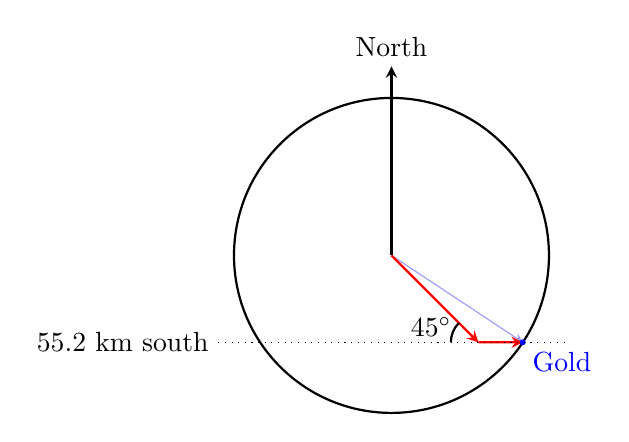
\begin{tikzpicture}[scale=1, >=stealth]

% Parameters
\def\R{2}                 % 100 km visual radius
\def\bearing{123.5}
\def\ysouth{-1.104}       % 55.2 km south (scaled)

% Origin
\coordinate (O) at (0,0);

% Gold
\coordinate (G) at ({\R*sin(\bearing)}, {\R*cos(\bearing)});

% Rob turning point: SE until y = gold y
\coordinate (R) at ({-\ysouth}, {\ysouth});

% Main circle
\draw[thick] (O) circle (\R);

% North arrow
\draw[->, thick] (O) -- (0,1.2*\R) node[above] {North};

% True bearing (faint)
\draw[blue!40, ->]
  (O) -- (G);

% Rob: first leg SE (135°)
\draw[thick, red, ->]
  (O) -- (R);

% Rob: second leg East (090°)
\draw[thick, red, ->]
  (R) -- (G);

% Gold
\filldraw[blue]
  (G) circle (0.03)
  node[below right] {Gold};

% Horizontal guide at 55.2 km south
\draw[dotted] (-2.2,{\ysouth}) -- (2.2,{\ysouth});
\node[left] at (-2.2,{\ysouth}) {$55.2\text{ km south}$};

% Interior turn angle at R (45°)
\draw[thick]
  (R) ++({0.35*cos(180)},{0.35*sin(180)})
  arc[start angle=180, end angle=135, radius=0.35];

\node at ($(R)+(-0.6,0.2)$) {$45^\circ$};

\end{tikzpicture}

Observe that the end of the final leg of the journey is at a point $55.19370 \; \text{km}$ South and $55.19370 \; \text{km}$ East. Using Pythagoras, the total distance for the first leg is:

$$
\sqrt{55.19370^2 + 55.19370^2} = 78.0557 \; \text{km} \quad \text{(nearest 10cm)}
$$

The second leg is the remaining East distance:

$$
83.38868 - 55.19370 = 28.2960 \; \text{km} \quad \text{(nearest 10cm)}
$$

Thus Rob's total distance is $78.0557 + 28.2960 = 106.35 \; \text{km} \quad \text{(nearest metre)}$

Which takes $106.35 \div 20 = 5.32 \; \text{days} \quad \text{(3.s.f)}$

And thus Rob arrives Roughly $1$ day and $15$ hours before Bob.

\item It should be clear that travelling as close to the $123.5^\circ$ bearing will achieve the fastest path.

One such Journey is as follows:
\begin{itemize}
    \item Travel $a$ km an a bearing of $124^\circ$ 
    \item Travel $a$ km on a bearing of $123^\circ$
\end{itemize}

Which forms an isosceles triangle with the base the path of the $123.5^\circ$ ``bearing", with apex angle $179^\circ$, and equal sides length $a$ km;

Thus applying the cosine rule:

$$
100^2 = a^2 + a^2 - 2 \cdot a \cdot a \cdot \cos(179^\circ) = (2-2\cdot \cos(179^\circ) \cdot a^2
$$

Thus

$$
a = \sqrt\frac{100^2}{2 - 2\cdot \cos(179^\circ)} = 50.00190 \; \text{km} \quad \text{(nearest cm)}
$$

And so the journey takes only a little (less than a minute!) longer than $5$ days, and thus even with a $7$ hour delay, will arrive before Rob, who needs $5$ days $7$ hours and $40$ minutes.

Proving the route is the quickest possible is left as an exercise, (hint - consider all triangles with base as in our journey, and apply Pythagoras' theorem. You may also want to consider the graph of $x^2 + (100-x)^2$).


\end{enumerate}

\newpage

\section{Challenge I: Integer Distances}

\begin{enumerate}
    \item \begin{enumerate}
        \item Rounding to the nearest km, Bob travels $55$ km South, leaving Bob $193.79$m North of the gold; and $83$ km East, leaving Bob $388.68$m West of the gold. Applying Pythagoras, Bob ends up $\sqrt{193.79^2 + 388.68^2} = 434 \; \text{m} \quad \text{(3.s.f)}$ from the gold.

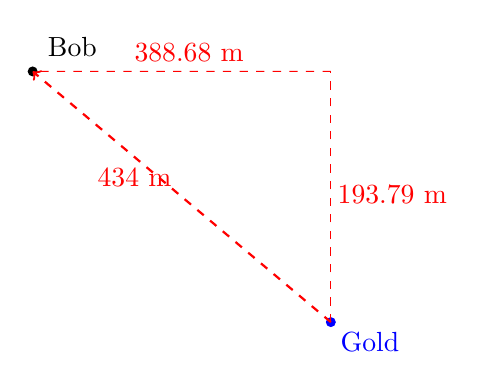
\begin{tikzpicture}[scale=0.6]
    % Coordinate system


    % Gold position
    \coordinate (G) at (0.38868,-0.19379);
    \fill(G) circle (3pt) node[above right=2pt] {Bob};
    
    \fill[blue] (6.7,-5.5) circle (3pt) node[below right] {Gold};
    
    % Displacement vectors
    \draw[red, dashed, thick, ->] (6.7,-5.5) -- (G) node[midway, above left] {434 m};
    \draw[red, dashed] (6.7,-5.5) -- (6.7,-0.19379);
    \draw[red, dashed] (6.7,-0.19379) -- (G);
    
    % Labels for displacements
    \node[red] at (8,-2.8) {193.79 m};
    \node[red] at (3.7,0.2) {388.68 m};
    
\end{tikzpicture}

        
        \item Rounding to the nearest km, Rob travels $78$km Southeast, and $28$km East. Observe that travelling Southeast constructs an isosceles right angled triangle, as the distance travelled South is equal to the distance travelled East. Denoting this distance $a$ we have that: $$78^2 = a^2 + a^2$$
        And thus $a = \sqrt{\frac{78^2}{2}} = 55.15432 \; \text{km} \quad \text{(nearest cm)}$

        So Rob travels $55.15432$ km South and $55.15432 + 28 = 83.15432 $ km East.

        This leaves Rob $55.19370-55.15432=0.0394$ km  (3.s.f) North of the gold, and $83.38868 - 83.15432 = 0.234$ km (3.s.f) West of the gold. Applying Pythagoras, he ends up $237$ meters away.

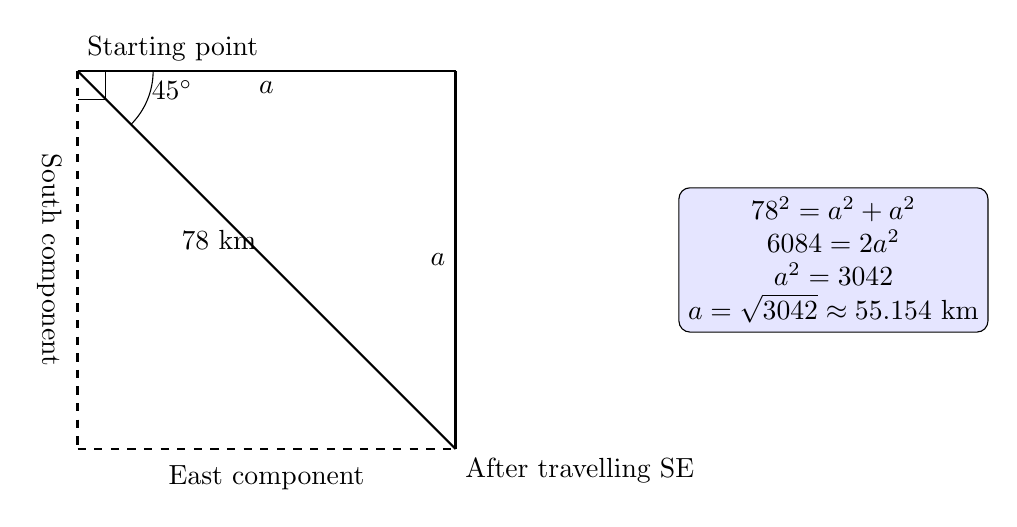
\begin{tikzpicture}[scale=1.2]
    % Define coordinates
    \coordinate (O) at (0,0);
    \coordinate (E) at (4,0);
    \coordinate (S) at (0,-4);
    \coordinate (SE) at (4,-4);
    
    % Draw the isosceles right triangle
    \draw[thick] (O) -- (SE) node[midway, above left] {$78$ km};
    \draw[thick] (O) -- (E) node[midway, below] {$a$};
    \draw[thick, dashed] (O) -- (S);
    \draw[thick] (E) -- (SE) node[midway, left] {$a$};
    \draw[thick, dashed] (S) -- (SE);
    
    % Right angle mark at origin
    \draw (0.3,0) -- (0.3,-0.3) -- (0,-0.3);
    
    % 45 degree angle mark
    \draw (0.8,0) arc (0:-45:0.8);
    \node at (1.0,-0.2) {$45^\circ$};
    
    % Label the sides
    \node at (2, -4.3) {East component};
    \node[rotate=-90] at (-0.3, -2) {South component};
    

    
    % Pythagoras equation
    \node[draw, rounded corners, fill=blue!10, align=center] at (8,-2) {
        $78^2 = a^2 + a^2$\\
        $6084 = 2a^2$\\
        $a^2 = 3042$\\
        $a = \sqrt{3042} \approx 55.154$ km
    };
    
    % Annotations
    \node[above right] at (O) {Starting point};
    \node[below right] at (SE) {After travelling SE};
    
\end{tikzpicture}

    \item The quickest journey, now rounded, becomes: \begin{itemize}
    \item Travel $50$ km an a bearing of $124^\circ$ 
    \item Travel $50$ km on a bearing of $123^\circ$
    \end{itemize}
    Applying the cosine rule as per the previous section, this covers:
    $$
    \sqrt{50^2 + 50^2 - 2 \cdot 50 \cdot 50 \cdot \cos(179^\circ)} = 99.99619 \; \text{km} \quad \text{(nearest cm)}
    $$
    As this also travels from the origin, at an angle of $123.5^\circ$ from North, we have that the distance from the gold is:
    $$
    100 - 99.99619 - 0.00381 \; \text{km} = 3.81 \; \text{m}
    $$
    \end{enumerate}

    Thus, neither you, Bob nor Rob end up within $1$m of the gold, and it remains buried.

    \item We consider the displacement East-West and South-North, setting East and North the positive directions respectively.

   We use right-angled trigonometry to resolve each leg into a vector $(x,y)$ indicating the East-West and South-North displacement, and see that (all to the nearest $\mu$m):

    \begin{itemize}
    \item $2$km on a bearing $179\degree$, $=(2 \cdot \sin(1^\circ), -2 \cdot \cos(1^\circ)) = (0.034904048, -1.999695390) $
    \item $2$km on a bearing of $000\degree$, $ = (0.00000000, 2.000000000)$
    \item $1$km on a bearing of $182\degree$, $ = (-\sin(2^\circ), -\cos(2^\circ)) = (-0.034899497, 0.999390827)$
    \item $1$km on a bearing of $000\degree$, $= (0.000000000,1.000000000)$
    \end{itemize}

    Which when combined result in a total displacement of:

    $$
    (2\cdot\sin(1^\circ) - \sin(2^\circ), 3-2\cdot \cos(1^\circ) - \cos(2^\circ)) = (0.000005316, 0.000913783)
    $$

    Which is $0.5316$cm East and $91.3783$cm North

    \item This is the same journey as the previous question, with all directions rotated $90^\circ$ anticlockwise. And thus the final outcome is: $0.5316$cm North and $91.3783$cm West. 

    We standardise this and write:
    $0.5316$cm North and $-91.3783$cm East. 

    \item Let $A$ be the number of repetitions of the 4 leg route from 2), and $B$ the number of repetitions of the 4 leg route from 3), considering the East-West and North-South components respectively, we derive the following simultaneous equations:

    \begin{align}
        0.000005316A - 0.000913783B &= 100 \cdot \sin(56.5^\circ) \\
        0.000913783A + 0.000005316B &= - 100 \cdot \cos(56.5^\circ) 
    \end{align}

    Which can be solved via substitution or elimination, to reduce numerical error, we introduce the following constants:

    \begin{align}
        \alpha &= 2\cdot\sin(1^\circ)-\sin(2^\circ) &&\approx 0.000005316\\
        \beta &= 3-2\cdot\cos(1^\circ)-\cos(2^\circ) &&\approx 0.000913783 
    \end{align}

Thus we have:

\begin{align}
    \alpha A - \beta B &= 100\cdot \sin(56.5^\circ) \\
    \beta A + \alpha B &= -100 \cdot \cos(56.5^\circ)
\end{align}

Which yields $A = \frac{100\cdot \sin(56.5^\circ)}{\alpha} +\frac{\beta B}{\alpha}$

Thus:

\begin{equation}
    \beta \cdot \left(\frac{100\cdot \sin(56.5^\circ)}{\alpha} +\frac{\beta B}{\alpha} \right) + \alpha B = -100 \cdot \cos(56.5^\circ)
\end{equation}

\begin{equation}
    \left( \frac{\beta^2}{\alpha} + \alpha \right) \cdot B = -100\cdot \cos(56.5^\circ) - \frac{100\beta\cdot\sin(56.5^\circ)}{\alpha}
\end{equation}

Thus:

\begin{equation}
B = \frac{-100\cdot \cos(56.5^\circ) - \frac{100\beta\cdot\sin(56.5^\circ)}{\alpha}}{ \frac{\beta^2}{\alpha} + \alpha} \approx -91604.77
\end{equation}

Then
\begin{equation}
A = \frac{100\cdot\sin(56.5^\circ)+\beta B}{\alpha} \approx -59868.41
\end{equation}

Observe that to achieve a negative value for $A$ and $B$ we have to reverse the direction of each bearing from 2) and 3). 

Since we may only take integer km steps, we thus complete $59868$ repeats of reverse of the path from 2), and $91605$ repeats of the reversed path from 3).

Using these rounded numbers we get that the East-West displacement is:


$$
\alpha \cdot -59868 + \beta \cdot 91605\approx 83.38879 \; \text{km} \quad \text{(nearest cm)}
$$

And the North-South displacement is:

$$
\beta \cdot -59868  + \alpha \cdot -91605 \approx -55.19333 \; \text{km} \quad \text{(nearest cm)}
$$

I.e $55.19333$ km South. 

We compare these to the true displacements of the gold:

East
$$
100 \cdot \sin (56.5^\circ) = 83.38868 \; \text{km} \quad \text{(nearest cm)}
$$

South
$$
100 \cdot \cos (56.5^\circ) = 55.19370 \; \text{km} \quad \text{(nearest cm)}
$$

Thus following this path, we end up roughly $11$ cm East, and roughly $37$ cm North of the gold's true location.

Applying Pythagoreans, this route ends up $\sqrt{37^2 + 11^2} \approx 39$ cm from the gold, and thus is close enough to find it.

Since each of the reversed routes involves travelling $2+2+1+1=6$ km, and we perform $59868+91605=151473$ total repeats, the total distance required is $151473\times 6 = 908838$ km, over twice the distance to the moon!

\item The simultaneous equations derived in the previous question can be applied to any $(x,y)$ coordinates, as we have two equations in two variables (exercise - what is the additional requirement to guarantee a solution?)

Thus we can always find real numbers $\hat{A},\hat{B}\in \mathbb{R}$ that solve them: 
\begin{align}
    \alpha \hat{A} - \beta \hat{B} &= x \\
    \beta \hat{A} + \alpha \hat{B} &= y
\end{align}


When rounded to the nearest integer, this adds an error of at most $0.5$ of an iteration, for the route from 2), and the route from 3).

Assuming a worst case scenario, this adds up to:

\begin{itemize}
\item $0.5136 \div 2 = 0.2568$ cm East-West (4.d.p)
\item $91.3783 \div 2 = 45.6892$ cm North-South (4.d.p)
\item another $45.6892$ cm East-West 
\item another $0.2568$ cm North-South
\end{itemize}

Which is less than $50$cm of error in each dimension, we see that:

$$
\sqrt{50^2 + 50^2} = 70.7\dots < 100
$$

And thus our final destination, with each step rounded to the nearest km remains within $1\text{m} = 100 \text{cm}$ of the gold, and thus is sufficient to find it.

\end{enumerate}

\section{Challenge II: Two Legs Only}

\begin{enumerate}
   \item Suppose we head out on a bearing of $090^\circ$ for $6000$ km for the first leg. 

   Then consider returning on a bearing of $269^\circ$, i.e. with a $1^\circ$ angle away from our original line.

   Consider a right angled triangle with base $5900$ and angle $1^\circ$, by right angled trigonometry, this has height:
   
   $$
   5900 \cdot \sin(1^\circ) \approx 102.97 \; \text{km}
   $$

      \begin{tikzpicture}[scale=2.0, >=stealth]

% Coordinates
\coordinate (O) at (0,0);
\coordinate (A) at (6,0);        % 6000 km east (scaled: 1000 km = 1 unit)
\coordinate (B) at (0.98,1.03);   % approximate return point with 1 degree offset

% Axes (optional, light)
\draw[->, gray!40] (-0.5,0) -- (7,0) node[right] {East};
\draw[->, gray!40] (0,-0.5) -- (0,2) node[above] {North};

% 100 km circle (scaled: 100 km = 0.1 units)
\draw[dashed, gray] (O) circle (0.98);
\node[gray] at (-0.35,0.15) {$100$ km};

% First leg
\draw[thick, blue, ->] (O) -- (A)
  node[midway, below] {$6000$ km, $090^\circ$};

% Return leg
\draw[thick, red, ->] (A) -- (B)
  node[midway, above right] {$269^\circ$};

% Right triangle projection
\draw[dashed] (A) -- (0.1,0);
\draw[dashed] (1.0,0) -- (B);

% Labels for triangle
\node at (3,0.15) {$5900$ km};
\node at (1.4,0.55) {$\approx 103$ km};

% Angle marker
\draw (A) ++(-0.8,0) arc (180:168:0.8);
\node at (5.1,0.11) {$1^\circ$};

% Points
\fill (O) circle (1pt) node[below left] {Start};
\fill (A) circle (1pt);
\fill (B) circle (1pt);

\end{tikzpicture}
   
   Which means that by the time we have returned to within $100$km East of the starting point, we are already over $100$km North, and will never be able to return to a position inside a circle radius $100$km of the origin,

   A similar argument holds for a return bearing of $268^\circ$, $267^\circ$ etc.

   And thus we have only one choice of return bearing: $270^\circ$, and then our return positions all lie due East of the origin

   By symmetry this argument holds for all initial bearings $ABC^\circ$, with only $XYZ^\circ$ the exact reverse bearing possible if we want to return within $100$ km of the start location

   \item Let $\theta$ be the non-reflex angle between the first and second leg of the journey, then the final distance from the start $D$ is given by the cosine rule:

   $$
   D^2 = M^2 + N^2 - 2 M N \cos(\theta)
   $$

   We require that $D^2 < 100^2$ to remain within $100$km of the start.

    See that $|M - N|^2 = (M-N)^2 = M^2 -2MN + N^2$

    Thus:

    $$
    D^2 = |M-N|^2 + 2MN - 2MN\cos(\theta) = |M-N|^2 + 2MN(1-\cos(\theta))
    $$


   Since $\cos(\theta) \leq 1 \quad \forall \theta$, we have that, $2MN(1-\cos (\theta))$ is always positive (or zero). Thus:

   $$
   D^2 \geq |M-N|^2
   $$

   Thus to ensure $D^2 < 100^2$ it must be the case that $|M-N|^2 < 100^2$, i.e.

   $$
   |M-N| \leq 100
   $$

   So $N$ must be within the range: $$[M-100, M+100]$$ as a necessary condition to return within $100$ km of the start. Not all such $N$ and $XYZ^\circ$ will do so, but those that do will definitely meet this criterion.

   \item From now on we omit journeys such as discussed in 1) since they can be replicated without a return leg, e.g. $6000$ km East and then $5950$km West ends up in the same location as travelling $50$km East. All journeys with $M>6000$ are not counted, as they replicate existing possibilities.

   Thus we have:
   \begin{itemize}
   \item At most $360$ options for $ABC^\circ$
   \item At most $6000$ options for $M$
   \item At most $360$ options for $XYZ^\circ$
   \item At most $203$ options for $N$ (by the previous question, $+2$ so the radius is $101$km which is a necessary condition to be within $1$m of the gold.) 
   \end{itemize}

    Not all of these combinations will end up within $101$km of the start, but all those unique journeys that do are included here.

    Thus there are at most $360\times6000\times360\times203 \approx 1.58\times10^{11}$ unique final destinations within $101$km of the start.

    \item Not necessarily, but possibly, since we would have to check each of the now finite possibilities and whether they end up within $1$ meter of the gold.

    \item 

    \begin{enumerate}
        \item Consider the first row of the table, $M\leq100$, in this case we opt to allow all possibilities:

        \begin{table}[h]
\centering
\begin{tabularx}{\textwidth}{|l|X|X|X|X|X|}
\hline
 & $ABC^{\circ}$ Option count &  $M$ in range &  $XYZ^{\circ}$ Option count per $M$ value (upper bound) & $N$ Option count per M value (upper bound) & Total journey option count for this $M$ range \\
\hline
$M \le 100$            &  $360$ & $101$ & $360$ & $203$ & $2.66 \times 10^9\\
\hline
$100 < M \le 500$      & & & & & \\
\hline
$500 < M \le 2000$     & & & & & \\
\hline
$2000 < M \le 6000$    & & & & & \\
\hline
\end{tabularx}
\end{table}


\item when $M>100$, we have left the circle in our first leg, so only have at most $180$ possible return bearings, since otherwise we would end up further away

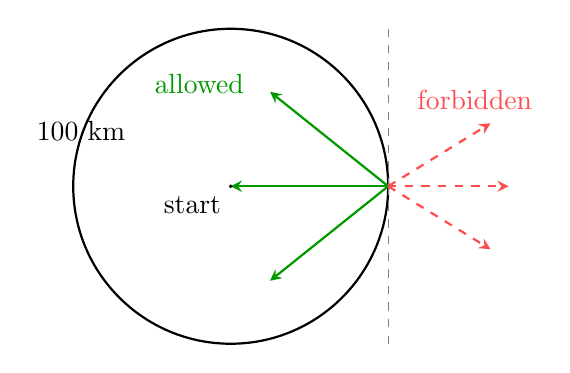
\begin{tikzpicture}[scale=1, >=stealth]

% Styles
\tikzset{
  point/.style={circle, fill, inner sep=0.5pt},
  allowed/.style={thick, green!60!black},
  forbidden/.style={thick, red!70, dashed}
}

% Coordinates
\coordinate (O) at (0,0);
\coordinate (A) at (2,0);   % exit point of circle (M > 100)
\coordinate (B) at (3.5,0); % further out on first leg

% Circle (radius 100 km)
\draw[thick] (O) circle (2);
\node at (-1.9,0.7) {$100$ km};



% Exit point
\node[point] at (A) {};


% Tangent line at exit point
\draw[dashed, gray] (A) -- ++(0,2);
\draw[dashed, gray] (A) -- ++(0,-2);

% Allowed return bearings (180 degrees)
\draw[allowed, ->] (A) -- ++(-1.5,1.2);
\draw[allowed, ->] (A) -- ++(-2,0);
\draw[allowed, ->] (A) -- ++(-1.5,-1.2);

\node[green!60!black] at (-0.4,1.3) {allowed};

% Forbidden return bearing
\draw[forbidden, ->] (A) -- ++(1.3,0.8);
\draw[forbidden, ->] (A) -- ++(1.53,0);
\draw[forbidden, ->] (A) -- ++(1.3,-0.8);
\node[red!70] at (3.1,1.1) {forbidden};

% Origin point
\node[point] at (O) {};
\node[below left] at (O) {start};

\end{tikzpicture}

So we set the $XYZ^\circ$ option count to $180$:

        \begin{table}[h]
\centering
\begin{tabularx}{\textwidth}{|l|X|X|X|X|X|}
\hline
 & $ABC^{\circ}$ Option count &  $M$ in range &  $XYZ^{\circ}$ Option count per $M$ value (upper bound) & $N$ Option count per M value (upper bound) & Total journey option count for this $M$ range \\
\hline
$M \le 100$            &  $360$ & $101$ & $360$ & $203$ & $2.66 \times 10^9\\
\hline
$100 < M \le 500$      & $360$ & $400$ & $180$ & $203$ & 5.26\times10^9 \\
\hline
$500 < M \le 2000$     & & & & & \\
\hline
$2000 < M \le 6000$    & & & & & \\
\hline
\end{tabularx}
\end{table}

\item For $M>500$, we consider a right angled triangle with base $400$ and height $100$, which then must have an angle of $\tan^{-1}(100/400) = 14.03^\circ$ as the return angle.

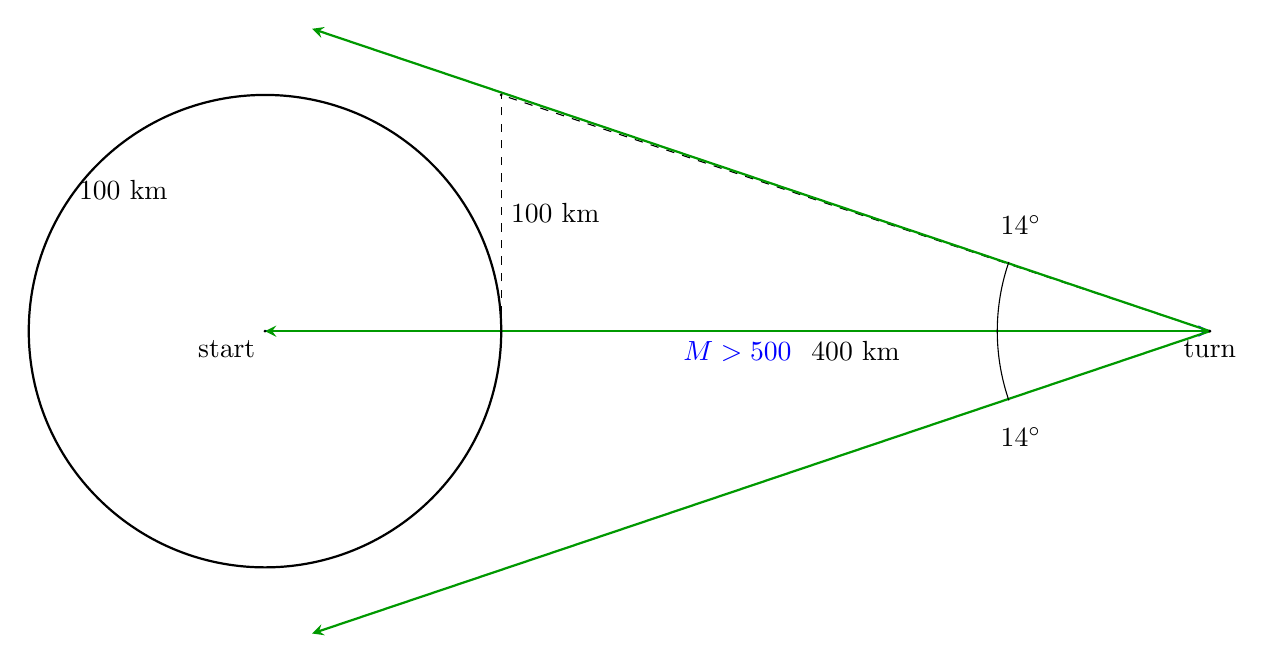
\begin{tikzpicture}[scale=3, >=stealth]

% Styles
\tikzset{
  point/.style={circle, fill, inner sep=0.4pt},
  allowed/.style={thick, green!60!black},
  triangle/.style={thick, dashed}
}

% Coordinates
\coordinate (O) at (0,0);
\coordinate (A) at (4,0);      % turning point (M > 500)
\coordinate (E) at (1,0);      % 100 km east of origin
\coordinate (N) at (1,1);      % 100 km north of that

% Small circle (radius 100 km)
\draw[thick] (O) circle (1);
\node at (-0.6,0.6) {$100$ km};

% First leg
\draw[thick, blue, ->] (O) -- (A)
  node[midway, below] {$M>500$};

% Dashed reference lines
\draw[dashed] (E) -- (N);        % 100 km north
\draw[dashed] (A) -- (N);        % slanted hypotenuse

% Right triangle edges
\draw[triangle] (A) -- (E);

% Labels
\node[below] at (2.5,0) {$400$ km};
\node[right] at (1,0.5) {$100$ km};

% Allowed return bearings (±14°)
\draw[allowed, ->] (A) -- ++(-3.8,1.28);
\draw[allowed, ->] (A) -- ++(-3.8,-1.28);
\draw[allowed, ->] (A) -- ++(-4,0);

% Angle marking
\draw (A) ++(-0.9,0) arc (180:161:0.9);
\node at (3.2,0.45) {$14^\circ$};

\draw (A) ++(-0.9,0) arc (180:199:0.9);
\node at (3.2,-0.45) {$14^\circ$};

% Points
\node[point] at (O) {};
\node[point] at (A) {};
\node[point] at (E) {};
\node[point] at (N) {};

% Labels
\node[below left] at (O) {start};
\node[below] at (A) {turn};

\end{tikzpicture}

And thus we have at most $14+14+1 = 29$ possible choices for our return bearing $XYZ^\circ$:

        \begin{table}[h]
\centering
\begin{tabularx}{\textwidth}{|l|X|X|X|X|X|}
\hline
 & $ABC^{\circ}$ Option count &  $M$ in range &  $XYZ^{\circ}$ Option count per $M$ value (upper bound) & $N$ Option count per M value (upper bound) & Total journey option count for this $M$ range \\
\hline
$M \le 100$            &  $360$ & $101$ & $360$ & $203$ & $2.66 \times 10^9\\
\hline
$100 < M \le 500$      & $360$ & $400$ & $180$ & $203$ & 5.26\times10^9 \\
\hline
$500 < M \le 2000$     & $360$ & $1500$ & $29$ & $203$ & $3.18\times 10^9$ \\
\hline
$2000 < M \le 6000$    & & & & & \\
\hline
\end{tabularx}
\end{table}

\item The argument for the case $M>2000$ is similar to the $M>500$, and we evaluate:

$$\tan^{-1}(100/1900) \approx 3.01$$

And thus we have at most $3+3+1=7$ options for the return bearing, and our complete table becomes:


        \begin{table}[h]
\centering
\begin{tabularx}{\textwidth}{|l|X|X|X|X|X|}
\hline
 & $ABC^{\circ}$ Option count &  $M$ in range &  $XYZ^{\circ}$ Option count per $M$ value (upper bound) & $N$ Option count per M value (upper bound) & Total journey option count for this $M$ range \\
\hline
$M \le 100$            &  $360$ & $101$ & $360$ & $203$ & $2.66 \times 10^9\\
\hline
$100 < M \le 500$      & $360$ & $400$ & $180$ & $203$ & 5.26\times10^9 \\
\hline
$500 < M \le 2000$     & $360$ & $1500$ & $29$ & $203$ & $3.18\times 10^9$ \\
\hline
$2000 < M \le 6000$    & $360$ & $4000$ & $7$ & $203$ & $2.05\times 10^9$ \\
\hline
\end{tabularx}
\end{table}
    \end{enumerate}


By summing the last column we see that there are at most:

$$
2.66\times 10^9 + 5.26\times 10^9 + 3.18\times 10^9 + 2.05 \times 10^9 = 1.32\times 10^{10}
$$

Possible endpoints for a two leg journey that finish within $101$km of the start.

\item 

The journey described is the same as the generic journey: 

\begin{itemize}
    \item Travel $M$km on a bearing of $ABC\degree$
    \item Travel $N$km on a bearing of $XYZ\degree$
\end{itemize}

Except with the order of the legs swapped. We see that this ends up in the same end point.

Observe that if a journey $M$, $ABC^\circ$, $N$, $XYZ^\circ$ does finish within $101$km of the start, then so will $N$, $XYZ^\circ$, $M$, $ABC^\circ$, and thus we can halve the upper bound from the previous question.

(There is some subtlety to this argument, since we first discard the journeys that end outside the radius to consider a true count with duplicates: $U'$, with $U'\leq U=1.32\times10^{10}$, then see that omitting the duplicates yields $\frac{U'}{2} \leq \frac{U}{2}$)

Thus we establish an upper bound on the number of two leg journeys that finish within $101$km of the starting point 

$$U = 6.6\times 10^9 < 10^{10}$$

\item $100$km is $10^5$m and thus the area is $10^{10}\pi$ square meters.

Consider the destination of each of the $6.6\times 10^9$ potential journeys, if they do finish inside the $100$km radius circle, they make accessible a circle of points radius $1$m from the endpoint, that is they cover an area of $\pi$ square meters.

So all the possibilities cover at most $6.6\times 10^9 \pi$ square meters, but this still leaves over $3 \times 10^9 \pi $ square meters, all the points inside of which are not accessible.

Thus some locations exist that cannot be reached within $1$m, following a two leg journey as described.

\item 

Naive attempt:

\newpage{}



\begin{minted}{python}

import math
from tqdm import tqdm

# -----------------------------
# PARAMETERS
# -----------------------------

# Gold location (km) — CHANGE THIS
GOLD_X = 83.38868
GOLD_Y = -55.19370

# Tolerance: 100 m = 0.1 km
TOL = 0.1

# Search limits
MAX_M = 6000
MAX_N_OFFSET = 101

# -----------------------------
# HELPER FUNCTIONS
# -----------------------------

def step(x, y, distance, bearing_deg):
    """
    Move distance (km) from (x, y) on a bearing in degrees.
    Bearings measured clockwise from North.
    """
    theta = math.radians(bearing_deg)
    dx = distance * math.sin(theta)
    dy = distance * math.cos(theta)
    return x + dx, y + dy


def in_gold_box(x, y):
    return (
        abs(x - GOLD_X) <= TOL and
        abs(y - GOLD_Y) <= TOL
    )

# -----------------------------
# BRUTE FORCE SEARCH
# -----------------------------

hits = []

for ABC in tqdm(range(360)):
    for M in tqdm(range(1, MAX_M + 1)):

        # First leg
        x1, y1 = step(0.0, 0.0, M, ABC)

        for XYZ in range(360):

            # Restrict N range
            for N in range(max(1, M - MAX_N_OFFSET), M + MAX_N_OFFSET + 1):

                # Second leg
                x2, y2 = step(x1, y1, N, XYZ)

                # Check if inside 100m box around gold
                if in_gold_box(x2, y2):
                    hits.append({
                        "ABC": ABC,
                        "M": M,
                        "XYZ": XYZ,
                        "N": N,
                        "x": x2,
                        "y": y2
                    })

# -----------------------------
# OUTPUT
# -----------------------------

print(f"Total solutions found: {len(hits)}")

for h in hits:
    print(
        f"ABC={h['ABC']:3d}, M={h['M']:4d}, "
        f"XYZ={h['XYZ']:3d}, N={h['N']:4d}, "
        f"x={h['x']:.4f}, y={h['y']:.4f}"
    )
\end{minted}


Unfortunately this would take over $42$ hours to run, due to the slowness of python, to circumvent this, use the Numpy library, with vectorisation, the following code takes roughly $40$ minutes to complete.
\newpage

\begin{minted}{python}

import numpy as np
from tqdm import tqdm

# -----------------------------
# PARAMETERS
# -----------------------------

# Gold location (km) — CHANGE THIS
GOLD_X = 83.38868
GOLD_Y = -55.19370

# Tolerance: 15 m = 0.015 km
TOL = 0.015

# Search limits
MAX_M = 6000
MAX_N_OFFSET = 101

# -----------------------------
# MORE MEMORY-EFFICIENT VERSION (still vectorized over M)
# -----------------------------

def find_solutions_vectorized_M():
    """
    Vectorized over M with chunked XYZ processing to manage memory.
    """
    all_abc = np.arange(360)
    all_xyz = np.arange(360)
    
    # Precompute trig
    sin_abc = np.sin(np.deg2rad(all_abc))
    cos_abc = np.cos(np.deg2rad(all_abc))
    sin_xyz = np.sin(np.deg2rad(all_xyz))
    cos_xyz = np.cos(np.deg2rad(all_xyz))
    
    all_M = np.arange(MAX_M + 1)
    max_N_len = 2 * MAX_N_OFFSET + 1
    
    hits = []
    
    # Process each ABC
    for abc_idx in tqdm(range(360), desc="Processing ABC"):

        abc = all_abc[abc_idx]
        sin_abc_val = sin_abc[abc_idx]
        cos_abc_val = cos_abc[abc_idx]
        
        # x1 and y1 for all M
        x1 = all_M * sin_abc_val
        y1 = all_M * cos_abc_val
        
        # N ranges for all M
        N_min = np.maximum(0, all_M - MAX_N_OFFSET)
        N_max = np.minimum(all_M + MAX_N_OFFSET, MAX_M + MAX_N_OFFSET)
        
        # Create array of N values for each M
        N_arrays = []
        valid_lengths = []
        
        for i, M in enumerate(all_M):
            if N_min[i] <= N_max[i]:
                N_range = np.arange(N_min[i], N_max[i] + 1)
                N_arrays.append(N_range)
                valid_lengths.append(len(N_range))
            else:
                N_arrays.append(np.array([], dtype=int))
                valid_lengths.append(0)
        
        # Process XYZ in chunks to manage memory
        xyz_chunk_size = 90 # Process 180 XYZ at a time
        for xyz_start in range(0, 360, xyz_chunk_size):
            xyz_end = min(360, xyz_start + xyz_chunk_size)
            xyz_chunk = all_xyz[xyz_start:xyz_end]
            
            sin_xyz_chunk = sin_xyz[xyz_start:xyz_end]
            cos_xyz_chunk = cos_xyz[xyz_start:xyz_end]
            
            # Process each M and its N range
            for m_idx, M in enumerate(all_M):
                if valid_lengths[m_idx] == 0:
                    continue
                    
                N_range = N_arrays[m_idx]
                L = len(N_range)
                
                # Vectorized over N and XYZ chunk
                # x2 shape: (L, xyz_chunk_size)
                x2 = x1[m_idx] + np.outer(N_range, sin_xyz_chunk)
                y2 = y1[m_idx] + np.outer(N_range, cos_xyz_chunk)
                
                # Check tolerance
                x_diff = np.abs(x2 - GOLD_X)
                y_diff = np.abs(y2 - GOLD_Y)
                mask = (x_diff <= TOL) & (y_diff <= TOL)
                
                # Get indices
                n_indices, xyz_chunk_indices = np.where(mask)
                
                for i in range(len(n_indices)):
                    N = N_range[n_indices[i]]
                    xyz = xyz_chunk[xyz_chunk_indices[i]]
                    
                    hits.append({
                        "ABC": abc,
                        "M": M,
                        "XYZ": xyz,
                        "N": N,
                        "x": x2[n_indices[i], xyz_chunk_indices[i]],
                        "y": y2[n_indices[i], xyz_chunk_indices[i]]
                    })
    
    return hits

# -----------------------------
# MAIN EXECUTION
# -----------------------------

if __name__ == "__main__":

    
    print("Running vectorized version (M dimension fully vectorized)...")
    hits = find_solutions_vectorized_M()
    
    # Output
    print(f"Total solutions found: {len(hits)}")
    
    for h in hits:  # Print solutions
        print(
            f"ABC={h['ABC']:3d}, M={h['M']:4d}, "
            f"XYZ={h['XYZ']:3d}, N={h['N']:4d}, "
            f"x={h['x']:.9f}, y={h['y']:.9f}"
        )

\end{minted}


Running this code finds all the points within $15$m of the gold:

\begin{minted}{bash}
Total solutions found: 82
ABC=  2, M=4832, XYZ=181, N=4885, x=83.379362620, y=-55.199514683
ABC=  2, M=4833, XYZ=181, N=4886, x=83.396809711, y=-55.199971551
ABC=  4, M=4937, XYZ=183, N=4987, x=83.388297091, y=-55.191773688
ABC= 18, M= 469, XYZ=187, N= 505, x=83.384951942, y=-55.190300436
ABC= 25, M= 230, XYZ=183, N= 264, x=83.385507752, y=-55.187406157
ABC= 34, M=5729, XYZ=213, N=5729, x=83.379112383, y=-55.187430591
ABC= 34, M=5730, XYZ=213, N=5730, x=83.393666251, y=-55.197063587
ABC= 35, M=1910, XYZ=212, N=1910, x=83.385198745, y=-55.191459067
ABC= 37, M= 819, XYZ=210, N= 819, x=83.386503962, y=-55.192322971
ABC= 40, M=1147, XYZ=215, N=1140, x=83.400250870, y=-55.180354232
ABC= 41, M= 383, XYZ=206, N= 383, x=83.374458883, y=-55.184350507
ABC= 46, M= 231, XYZ=201, N= 231, x=83.384497533, y=-55.190994945
ABC= 60, M= 505, XYZ=229, N= 469, x=83.384035787, y=-55.191684597
ABC= 61, M= 106, XYZ=185, N= 107, x=83.384024483, y=-55.203012950
ABC= 62, M= 107, XYZ=186, N= 106, x=83.395375330, y=-55.185863691
ABC= 64, M= 264, XYZ=222, N= 230, x=83.381588760, y=-55.193327107
ABC= 64, M=4987, XYZ=243, N=4937, x=83.386698976, y=-55.194188177
ABC= 66, M=4885, XYZ=245, N=4832, x=83.390333623, y=-55.182939306
ABC= 66, M=4886, XYZ=245, N=4833, x=83.397571294, y=-55.198820924
ABC= 73, M= 178, XYZ=219, N= 138, x=83.376032597, y=-55.203979240
ABC= 74, M=  77, XYZ=173, N=  77, x=83.401090029, y=-55.201977278
ABC= 76, M=  74, XYZ=171, N=  74, x=83.378034157, y=-55.186716930
ABC= 90, M= 533, XYZ=263, N= 453, x=83.376593306, y=-55.206812563
ABC= 94, M=  24, XYZ=132, N=  80, x=83.393123244, y=-55.204603879
ABC= 98, M= 500, XYZ=272, N= 412, x=83.385013639, y=-55.207957839
ABC=100, M=1234, XYZ=278, N=1143, x=83.376364645, y=-55.206996844
ABC=105, M= 700, XYZ=282, N= 606, x=83.390632358, y=-55.178846936
ABC=108, M= 110, XYZ=225, N=  30, x=83.403013357, y=-55.205072817
ABC=113, M= 620, XYZ=291, N= 522, x=83.384026509, y=-55.185230001
ABC=115, M=  80, XYZ=153, N=  24, x=83.400394957, y=-55.193617520
ABC=122, M=  25, XYZ=124, N=  75, x=83.379020346, y=-55.187449366
ABC=122, M= 103, XYZ=261, N=   4, x=83.398200542, y=-55.207422076
ABC=123, M=  49, XYZ=124, N=  51, x=83.375774030, y=-55.206150793
ABC=123, M=  50, XYZ=124, N=  50, x=83.385407025, y=-55.191596924
ABC=123, M=  75, XYZ=125, N=  25, x=83.379093703, y=-55.187338535
ABC=123, M= 150, XYZ=302, N=  50, x=83.398180384, y=-55.199892041
ABC=124, M=  50, XYZ=123, N=  50, x=83.385407025, y=-55.191596924
ABC=124, M=  51, XYZ=123, N=  49, x=83.375774030, y=-55.206150793
ABC=124, M=  75, XYZ=122, N=  25, x=83.379020346, y=-55.187449366
ABC=124, M= 150, XYZ=305, N=  50, x=83.398033669, y=-55.200113703
ABC=125, M=  25, XYZ=123, N=  75, x=83.379093703, y=-55.187338535
ABC=132, M=  80, XYZ= 94, N=  24, x=83.393123244, y=-55.204603879
ABC=134, M= 620, XYZ=316, N= 522, x=83.379006830, y=-55.192813908
ABC=142, M= 700, XYZ=325, N= 606, x=83.375712299, y=-55.201388686
ABC=149, M= 500, XYZ=335, N= 412, x=83.400313618, y=-55.184842092
ABC=153, M=  24, XYZ=115, N=  80, x=83.400394957, y=-55.193617520
ABC=171, M=  74, XYZ= 76, N=  74, x=83.378034157, y=-55.186716930
ABC=171, M=1122, XYZ=355, N=1057, x=83.395849691, y=-55.208522265
ABC=173, M=  77, XYZ= 74, N=  77, x=83.401090029, y=-55.201977278
ABC=181, M=4885, XYZ=  2, N=4832, x=83.379362620, y=-55.199514683
ABC=181, M=4886, XYZ=  2, N=4833, x=83.396809711, y=-55.199971551
ABC=183, M= 264, XYZ= 25, N= 230, x=83.385507752, y=-55.187406157
ABC=183, M=4987, XYZ=  4, N=4937, x=83.388297091, y=-55.191773688
ABC=185, M= 107, XYZ= 61, N= 106, x=83.384024483, y=-55.203012950
ABC=186, M= 106, XYZ= 62, N= 107, x=83.395375330, y=-55.185863691
ABC=187, M= 505, XYZ= 18, N= 469, x=83.384951942, y=-55.190300436
ABC=201, M= 231, XYZ= 46, N= 231, x=83.384497533, y=-55.190994945
ABC=206, M= 383, XYZ= 41, N= 383, x=83.374458883, y=-55.184350507
ABC=210, M= 819, XYZ= 37, N= 819, x=83.386503962, y=-55.192322971
ABC=212, M=1910, XYZ= 35, N=1910, x=83.385198745, y=-55.191459067
ABC=213, M=5729, XYZ= 34, N=5729, x=83.379112383, y=-55.187430591
ABC=213, M=5730, XYZ= 34, N=5730, x=83.393666251, y=-55.197063587
ABC=215, M=1140, XYZ= 40, N=1147, x=83.400250870, y=-55.180354232
ABC=219, M= 138, XYZ= 73, N= 178, x=83.376032597, y=-55.203979240
ABC=222, M= 230, XYZ= 64, N= 264, x=83.381588760, y=-55.193327107
ABC=225, M=  30, XYZ=108, N= 110, x=83.403013357, y=-55.205072817
ABC=229, M= 469, XYZ= 60, N= 505, x=83.384035787, y=-55.191684597
ABC=243, M=4937, XYZ= 64, N=4987, x=83.386698976, y=-55.194188177
ABC=245, M=4832, XYZ= 66, N=4885, x=83.390333623, y=-55.182939306
ABC=245, M=4833, XYZ= 66, N=4886, x=83.397571294, y=-55.198820924
ABC=261, M=   4, XYZ=122, N= 103, x=83.398200542, y=-55.207422076
ABC=263, M= 453, XYZ= 90, N= 533, x=83.376593306, y=-55.206812563
ABC=272, M= 412, XYZ= 98, N= 500, x=83.385013639, y=-55.207957839
ABC=278, M=1143, XYZ=100, N=1234, x=83.376364645, y=-55.206996844
ABC=282, M= 606, XYZ=105, N= 700, x=83.390632358, y=-55.178846936
ABC=291, M= 522, XYZ=113, N= 620, x=83.384026509, y=-55.185230001
ABC=302, M=  50, XYZ=123, N= 150, x=83.398180384, y=-55.199892041
ABC=305, M=  50, XYZ=124, N= 150, x=83.398033669, y=-55.200113703
ABC=316, M= 522, XYZ=134, N= 620, x=83.379006830, y=-55.192813908
ABC=325, M= 606, XYZ=142, N= 700, x=83.375712299, y=-55.201388686
ABC=335, M= 412, XYZ=149, N= 500, x=83.400313618, y=-55.184842092
ABC=355, M=1057, XYZ=171, N=1122, x=83.395849691, y=-55.208522265
\end{minted}


We then can plot them to see if the gold will be found:

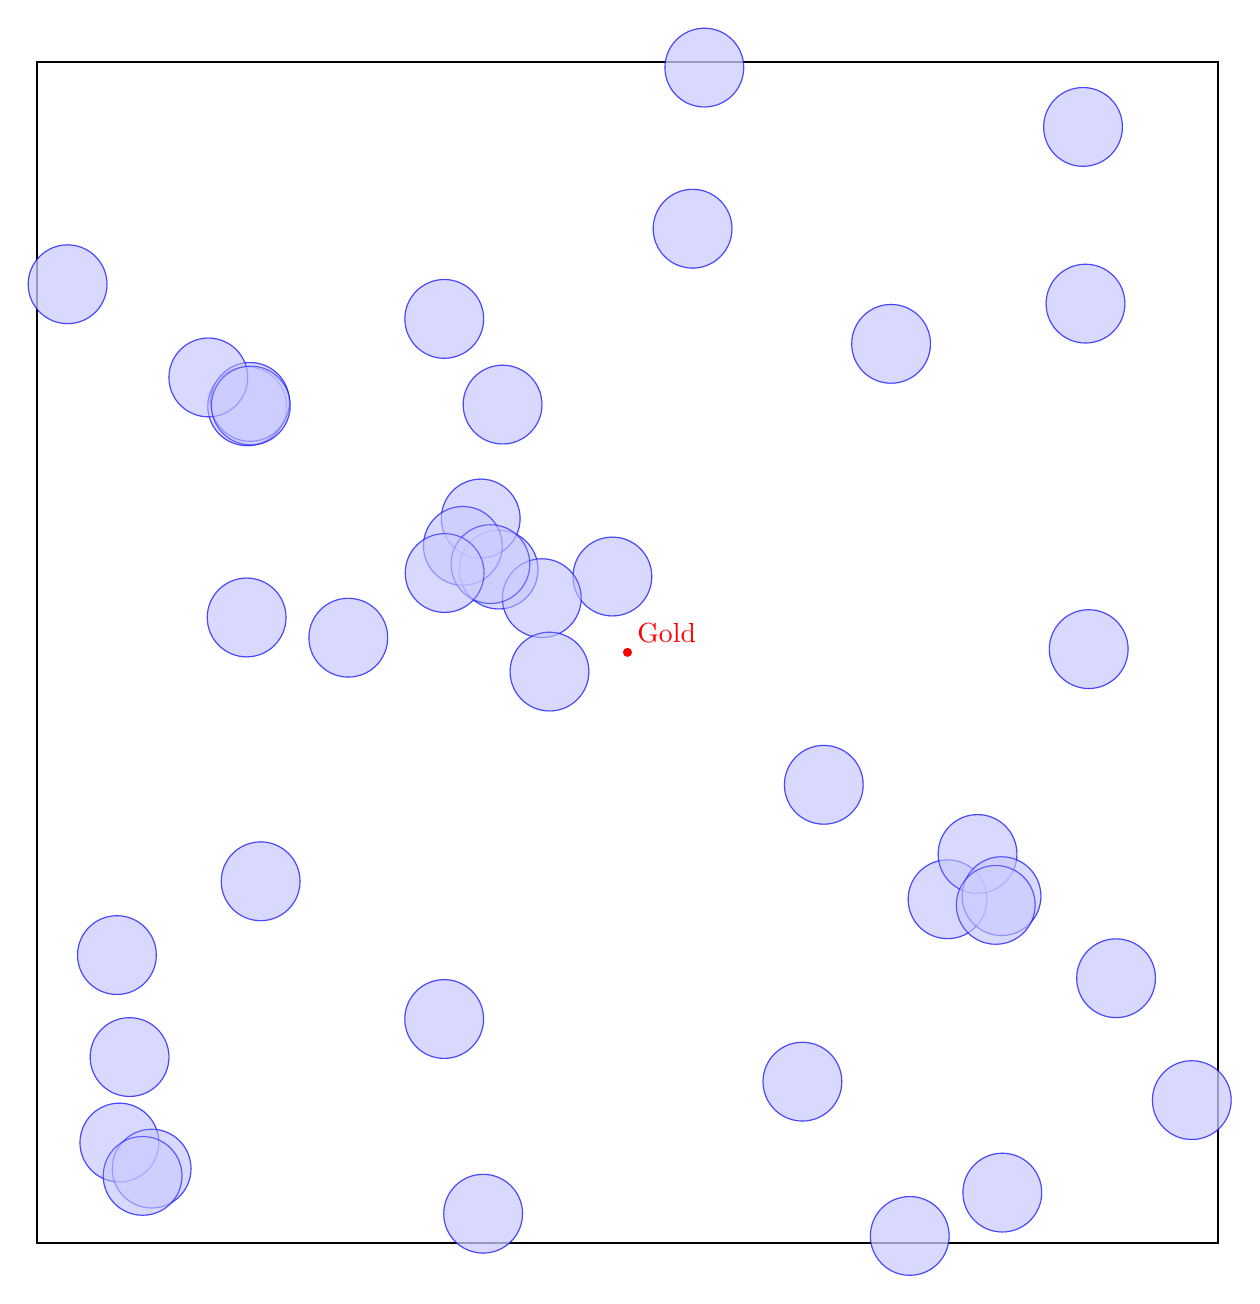
\begin{tikzpicture}[scale=0.5]
    %----------------------------------------
    % GOLD LOCATION (0,0 after translation)
    %----------------------------------------
    \coordinate (gold) at (0,0);

    % 30 m × 30 m square (±15 m)
    \draw[thick] (-15,-15) rectangle (15,15);

    % Mark gold point
    \filldraw[red] (gold) circle (0.1) node[above right]{Gold};

    % 1 m radius
    \def\r{1}

    %----------------------------------------
    % Candidate points (translated and km→m)
    % X_m = (X - 55.19370)*1000
    % Y_m = (Y + 83.38868)*1000
    %----------------------------------------

    \foreach \x/\y in {
      % FORMAT: x_m / y_m
        -9.31737999999882/-5.81468299999699,
8.12971100000937/-6.27155099999754,
-0.382908999995379/1.92631200000193,
-3.72805799999298/3.39956399999863,
-3.17224799999849/6.29384300000169,
-9.56761699998765/6.26940899999795,
4.98625100000538/-3.36358700000261,
-3.48125499999696/2.24093300000305,
-2.17603799998756/1.37702899999681,
11.5708699999999/13.3457680000006,
-14.2211169999911/9.34949300000198,
-4.18246699999258/2.70505499999985,
-4.64421299999174/2.01540300000147,
-4.65551699998912/-9.31295000000176,
6.69532999999944/7.83630899999821,
-7.09123999999406/0.372892999997987,
-1.98102399998845/-0.488177000001144,
1.65362300000993/10.7606939999982,
8.89129400000854/-5.12092400000341,
-12.6474029999883/-10.2792400000027,
12.4100290000086/-8.27727800000133,
-10.6458429999918/6.98306999999687,
-12.08669399999/-13.112563,
4.44324400000085/-10.9038789999971,
-3.66636100000051/-14.2578390000025,
-12.3153549999984/-13.2968440000027,
1.95235800001115/14.8530640000004,
14.3333570000124/-11.3728170000016,
-4.65349099999912/8.46999899999901,
11.7149570000095/0.0824800000032155,
-9.65965399998936/6.25063399999704,
9.52054200000418/-13.7220760000005,
-12.9059699999914/-12.4507929999993,
-3.27297499998735/2.10307599999737,
-9.58629699999847/6.36146499999768,
9.50038400000608/-6.19204099999848,
-3.27297499998735/2.10307599999737,
-12.9059699999914/-12.4507929999993,
-9.65965399998936/6.25063399999704,
9.35366900000645/-6.41370299999977,
-9.58629699999847/6.36146499999768,
4.44324400000085/-10.9038789999971,
-9.67316999999923/0.886092000001781,
-12.9677009999938/-7.68868600000161,
11.6336180000047/8.85790800000308,
11.7149570000095/0.0824800000032155,
-10.6458429999918/6.98306999999687,
7.16969100000142/-14.8222649999994,
12.4100290000086/-8.27727800000133,
-9.31737999999882/-5.81468299999699,
8.12971100000937/-6.27155099999754,
-3.17224799999849/6.29384300000169,
-0.382908999995379/1.92631200000193,
-4.65551699998912/-9.31295000000176,
6.69532999999944/7.83630899999821,
-3.72805799999298/3.39956399999863,
-4.18246699999258/2.70505499999985,
-14.2211169999911/9.34949300000198,
-2.17603799998756/1.37702899999681,
-3.48125499999696/2.24093300000305,
-9.56761699998765/6.26940899999795,
4.98625100000538/-3.36358700000261,
11.5708699999999/13.3457680000006,
-12.6474029999883/-10.2792400000027,
-7.09123999999406/0.372892999997987,
14.3333570000124/-11.3728170000016,
-4.64421299999174/2.01540300000147,
-1.98102399998845/-0.488177000001144,
1.65362300000993/10.7606939999982,
8.89129400000854/-5.12092400000341,
9.52054200000418/-13.7220760000005,
-12.08669399999/-13.112563,
-3.66636100000051/-14.2578390000025,
-12.3153549999984/-13.2968440000027,
1.95235800001115/14.8530640000004,
-4.65349099999912/8.46999899999901,
9.50038400000608/-6.19204099999848,
9.35366900000645/-6.41370299999977,
-9.67316999999923/0.886092000001781,
-12.9677009999938/-7.68868600000161,
11.6336180000047/8.85790800000308,
7.16969100000142/-14.8222649999994
    }{
       \filldraw[blue, fill=blue!20, opacity=0.5] (\x,\y) circle (\r);
    }

\end{tikzpicture}


And thus see that the gold cannot be found via a two step journey

\item One journeys end up within $2$m of the gold

\begin{itemize}
    \item $4937$km on a bearing of $004^\circ$, then $4987$ on a bearing of $183^\circ$
\end{itemize}

Which finishes in the following coordinates:


$$
(4937\cdot \sin(4^\circ) - 4987\cdot \sin(3^\circ), 4937 \cdot\cos(4^\circ) - 4987 \cdot \cos(3^\circ) ) = (83.38830, -55.19177)
$$

\end{enumerate}

\end{document}
